\newpage
\thispagestyle{fancy}

\section{La modélisation numérique de milieux urbains}

La modélisation numérique de milieux urbains correspond à la génération d'une représentation virtuelle d'un bâtiment ou d'une ville entière, représentation qui peut intégrer de nombreux aspects comme la géométrie (forme des bâtiments), la sémantique (différencier un arbre d'un trottoir et d'un toit), l'utilisation de textures pour améliorer le réalisme visuel du modèle.
\begin{figure}[H]
  \centering
   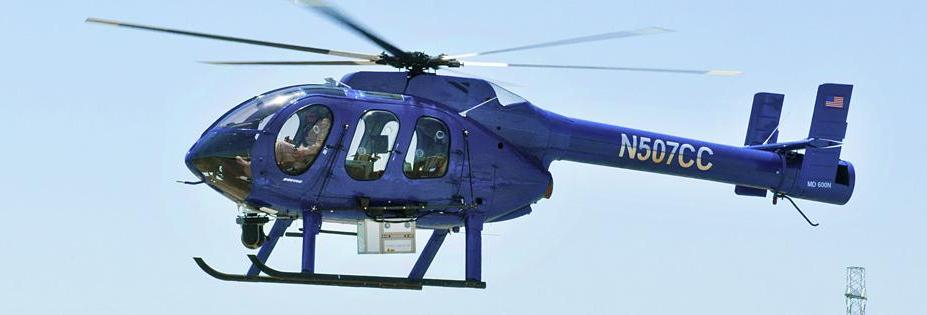
\includegraphics[width=7cm]{lidar-aero.jpg}
   \caption{Exemple de LIDAR aéroporté}
   \label{lidar}
\end{figure}
Ce domaine a été appréhendé d'un grand nombre d'approches, d'une part par les différents aspects évoqués ci-dessus, eux-mêmes déclinés sur un certains nombre de critères : quelle précision pour la reconstruction géométrique (à la rue près, au banc près, au buisson près  ?), quelle distinction sémantique (combien de classes différentes ?), quelles hypothèses sont faites (les murs sont forcément verticaux, un arbre ne peut pas dépasser 10m de hauteur) ?
D'autre part, les méthodes peuvent être automatisées ou comporter une partie de travail manuel, par exemple dans le choix de paramètres, ou dans la détection des erreurs. Certains travaux, comme ceux de Poullis \& You \cite{PY}, montrent la possibilité de reconstruire des villes entières à partir de nuages de points acquis par LIDAR aéroporté (Figure \ref{baltimore}).
\begin{figure}[H]
  \centering
   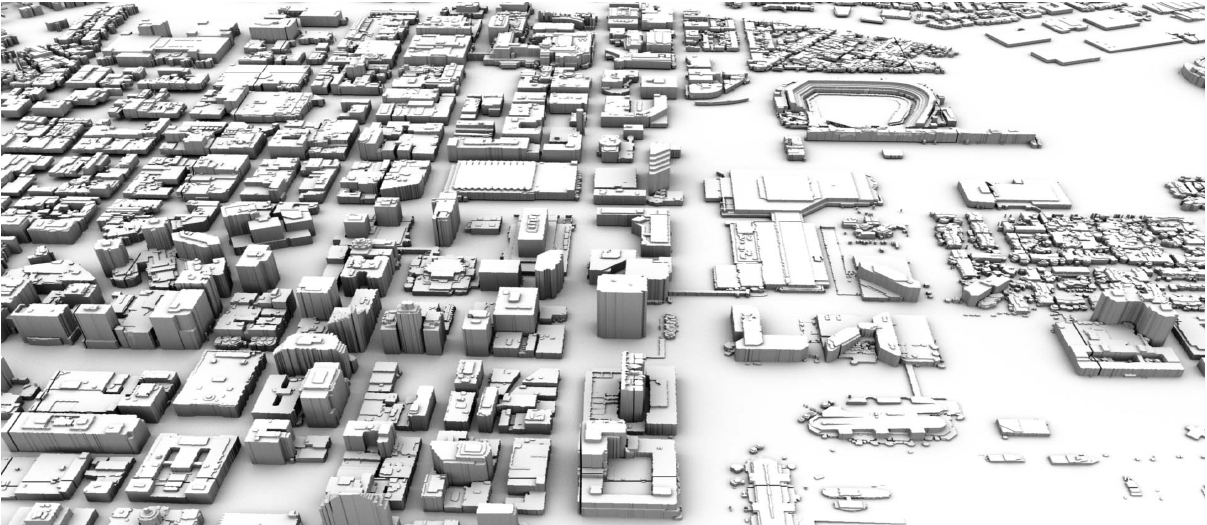
\includegraphics[width=\textwidth]{baltimore.png}
   \caption{Reconstruction 3D de la ville de Baltimore}
   \label{baltimore}
\end{figure}